%!TEX root = ../master.tex"`


\chapter{Proposed Trading Strategy}

In the data, almost all of profits are driven by the extremely unusual Asset2. A strategy that would have performed well would therefore have been a strategy centered on Asset2, or more general a momentum-like trading strategy that would have invested in stocks that have performed well in the past. This is of course easy to say in hindsight. Frankly, I don't think I could be very confident in recommending something other than a simple buy-and-hold strategy (maybe improved by some more elegant ways to optimally balance risks and profits in the portfolio). But then again this is why I am applying to this job: I am eager to learn more. 

There is, however, a couple of things that I have tried and some analyses I have run that are interesting in and of themselves. 

\section{General process for deriving a strategy}
\subsection{Data Preparation and Visualization}
I have split the data in training and test data set. I've done this for a couple of split dates, but present only the results for a training period of the first 1500 observations. As an initial step I extracted log returns and made sure that all time series are stationary see results\slash train\_stationarity.csv with the Augmented Dickey-Fuller test. 

Then I plotted the data. It can be seen in Figure \ref{1} that everything is dominated by Asset2. Plots for the full time series can be found in results\slash results\_full\_ts.  

\begin{figure}[h!]
    %\figuretitle{Stock Prices}
    \centering
    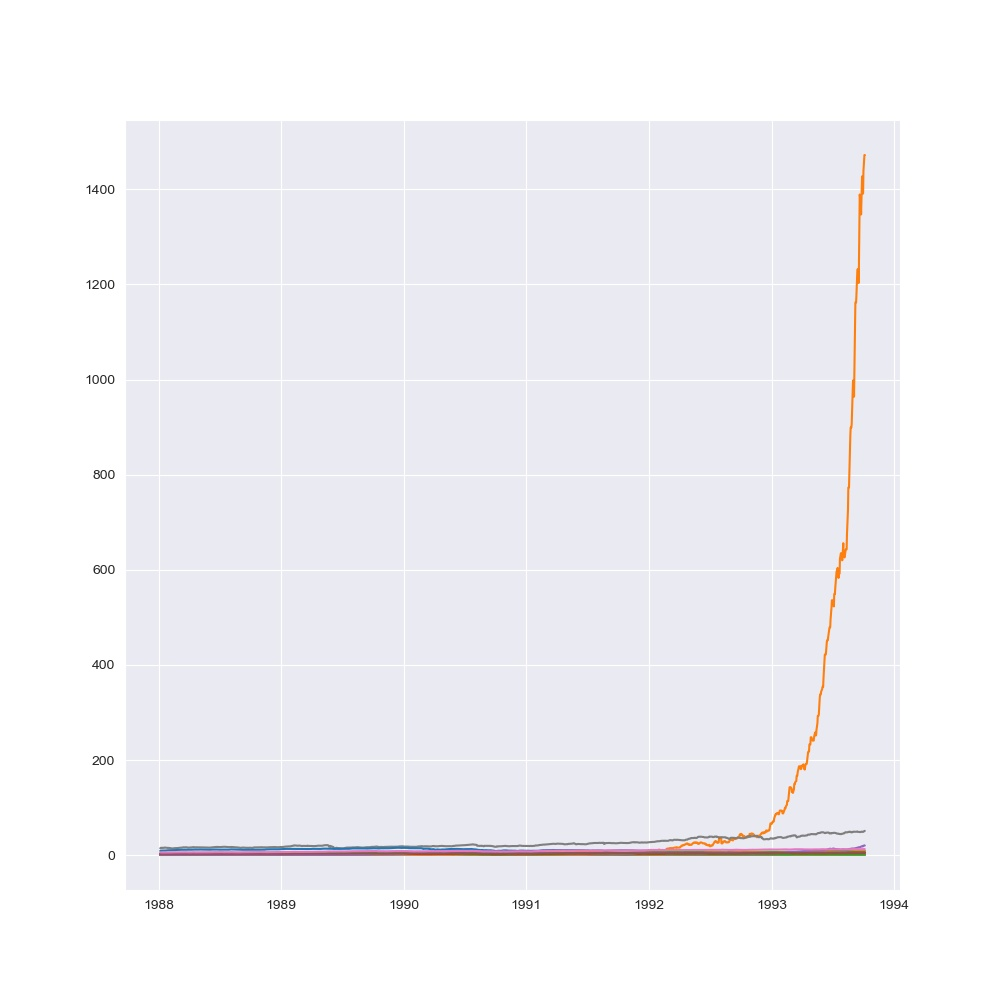
\includegraphics[width=0.48\textwidth]{../results/train_all_assets.jpg}
    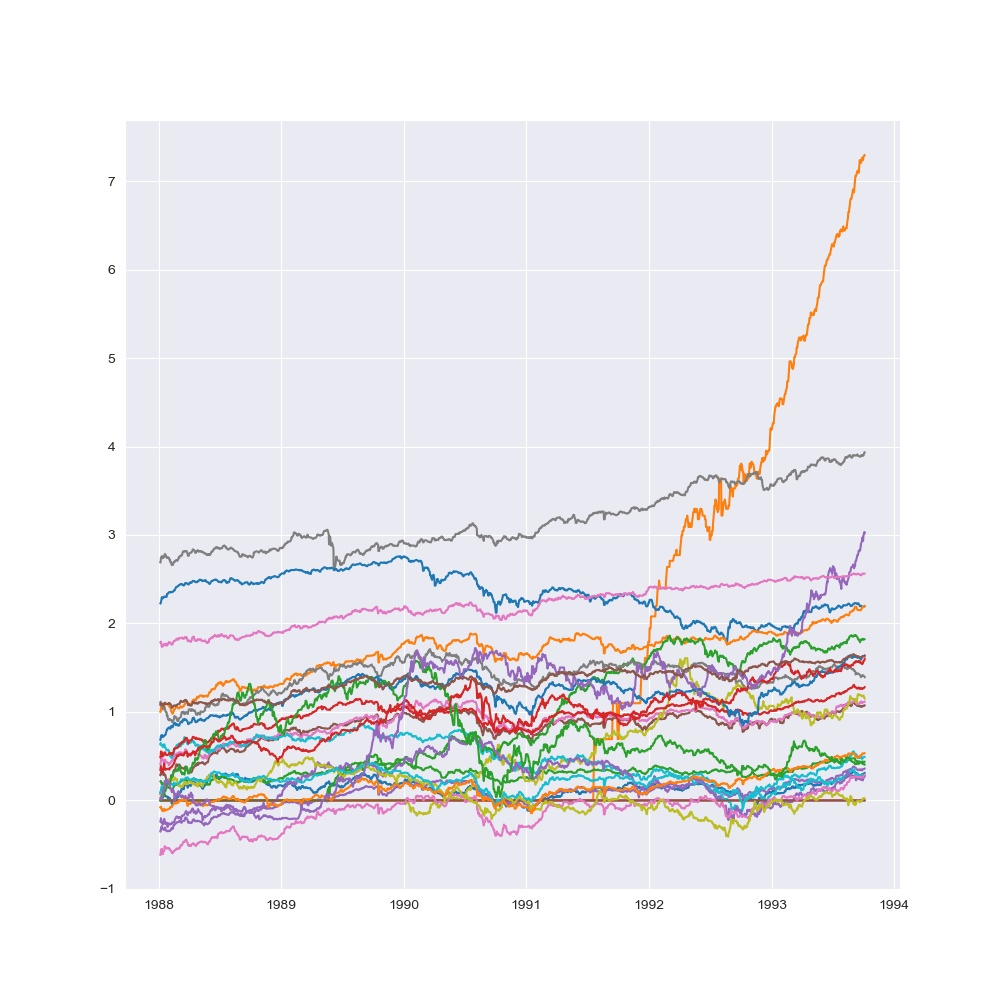
\includegraphics[width=0.48\textwidth]{../results/train_all_assets_logged.jpg}
    \caption{All Assets first 1500 obs}
    \label{1}
  
\end{figure}{}

\subsection{Look at Autocorrelations}
As can be seen in results\slash all\_autocorr\_log\_returns.jpg, log returns of the assets generally do not exhibit large amounts of autocorrelation. While it is of course possible to fit different time series models to the data I do not feel confident that I would not simply overfit to past observations. I have also looked at automatically selected arma orders (see results\slash train\_select\_arma\_order.csv). One can see that BIC values for the different orders do hardly change. I therefore have little confidence in the ARMA orders automatically chosen. I nevertheless implemented a trading strategy based on time series predictions. Right now it only looks at ARMA(1,1)-models, but it can be easily replaced by an auto-ARMA model. This trading strategy performs very poorly right now. One can adapt the threshold value in the trade-method of the python object, but I still have little confidence in this strategy and implemented it rather as a proof of principle. 


\subsection{Look at Cointegration}
Extensive literature suggests one can use cointegrated time series to construct a trading strategy that profits from the fact that time series move together. I tried all combinations of the time series and found combinations with p-values smaller than 0.05. However, none of them remained after adjusting for the testing of (sum(1, ..., 26) * 2) = 702 combinations. Also cointegration values differed greatly for different lengths of the time series. With more time, I would have liked to have a more thorough look at this. I did not implement a cointegration based strategy, because this would have meant focusing only on pairs of stocks instead of the entire portfolio. 

\subsection{Look at Conditional Heteroskedasticity}
As can be seen in results\slash train\_all\_autocorr\_squared\_log\_returns.jpg, the assets exhibit Conditional Heteroskedasticity. The squared log returns are oftentimes autocorrelated at lag 1, 5, 10. One could therefore model risks according to predicted variations in future returns. With more time, I would have looked into this to devise a trading strategy that uses this for risk management. 



\chapter{Results of the implemented trading strategies}

\section{Results for the training period}
Results are shown in Figure \ref{2}. The momentum based strategy is by far the best, however it is not able to outperform a buy-and-hold strategy. Figure \ref{3} shows a sanity check with the Assets 2 and 25 removed. Again, both mean reversion and momentum trading perform worse than the baseline. 


\begin{figure}[h!]
    %\figuretitle{Stock Prices}
    \centering
    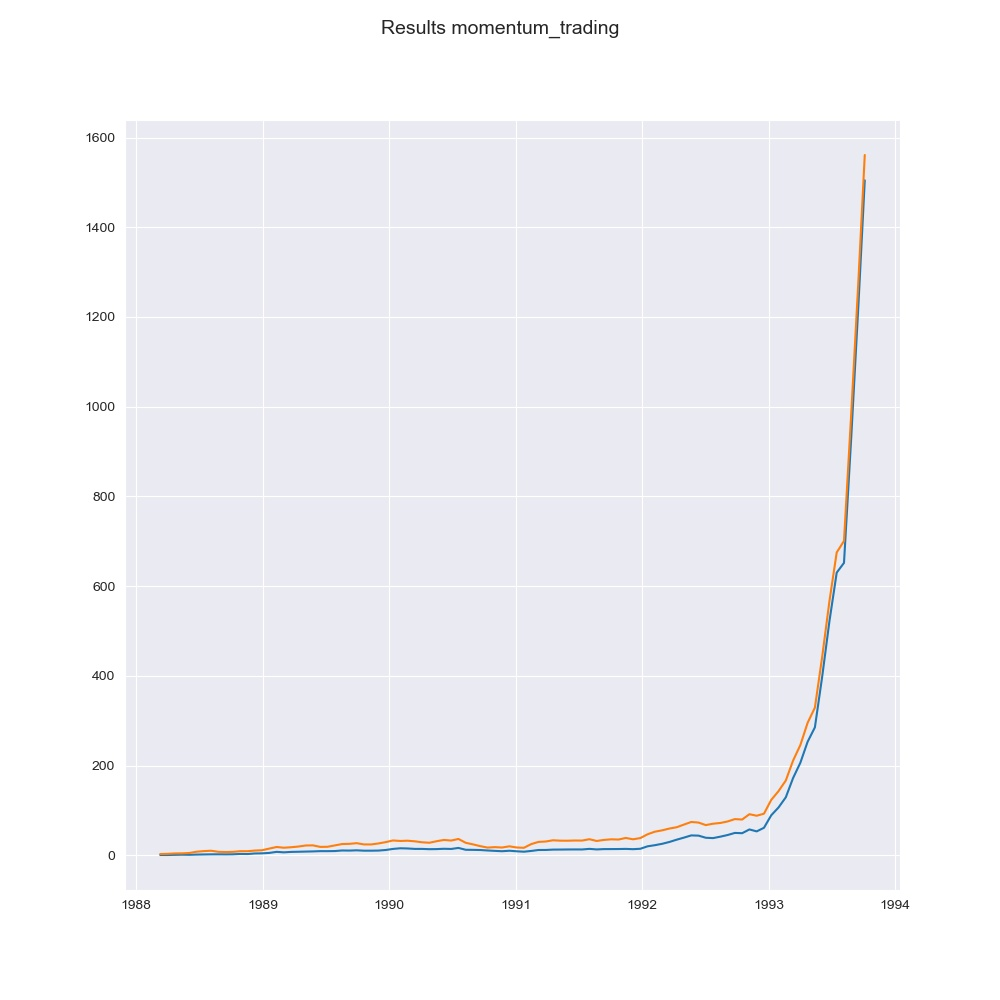
\includegraphics[width=0.48\textwidth]{../results/train_momentum_trading_results.jpg}
    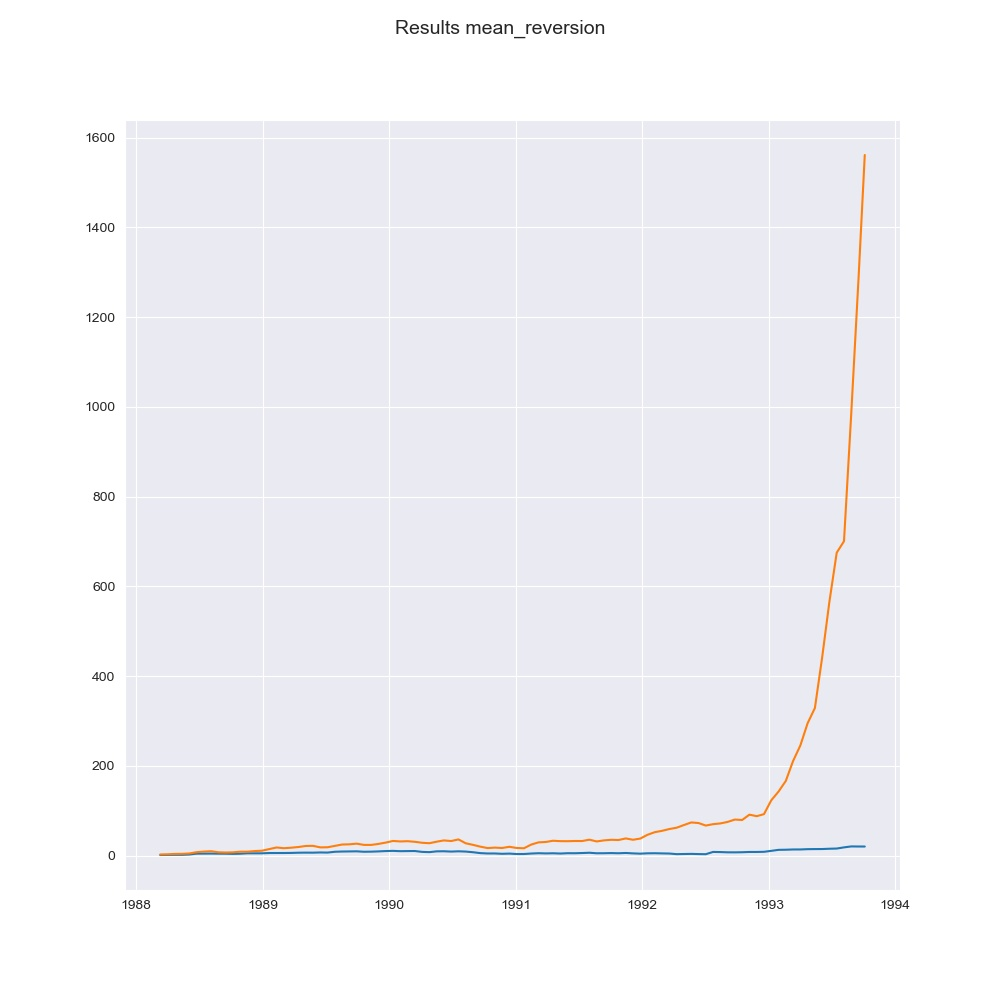
\includegraphics[width=0.48\textwidth]{../results/train_mean_reversion_results.jpg}

    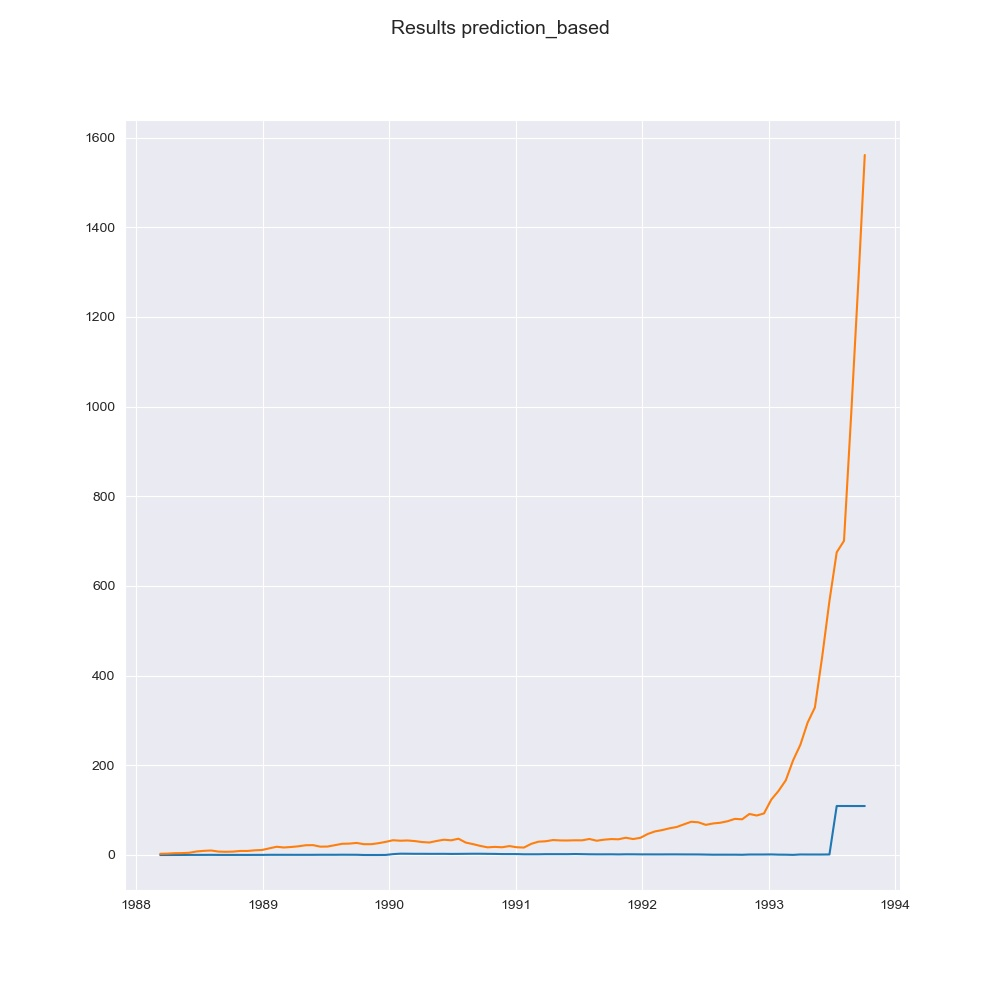
\includegraphics[width=0.48\textwidth]{../results/train_prediction_based_results.jpg}

    \caption{Results first 1500 obs, baseline in orange}
    \label{2}
  
\end{figure}{}

\begin{figure}[h!]
    %\figuretitle{Stock Prices}
    \centering
    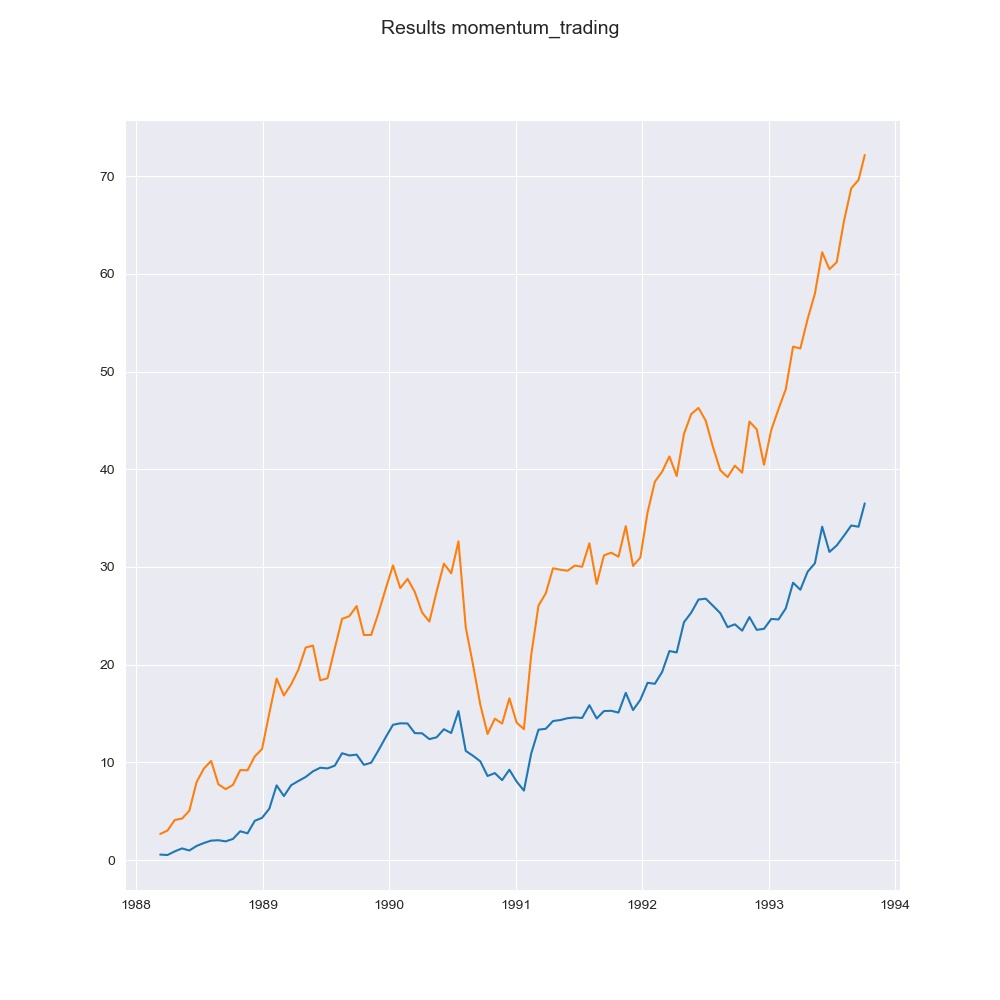
\includegraphics[width=0.48\textwidth]{../results/train_outliers_removed_momentum_trading_results.jpg}
    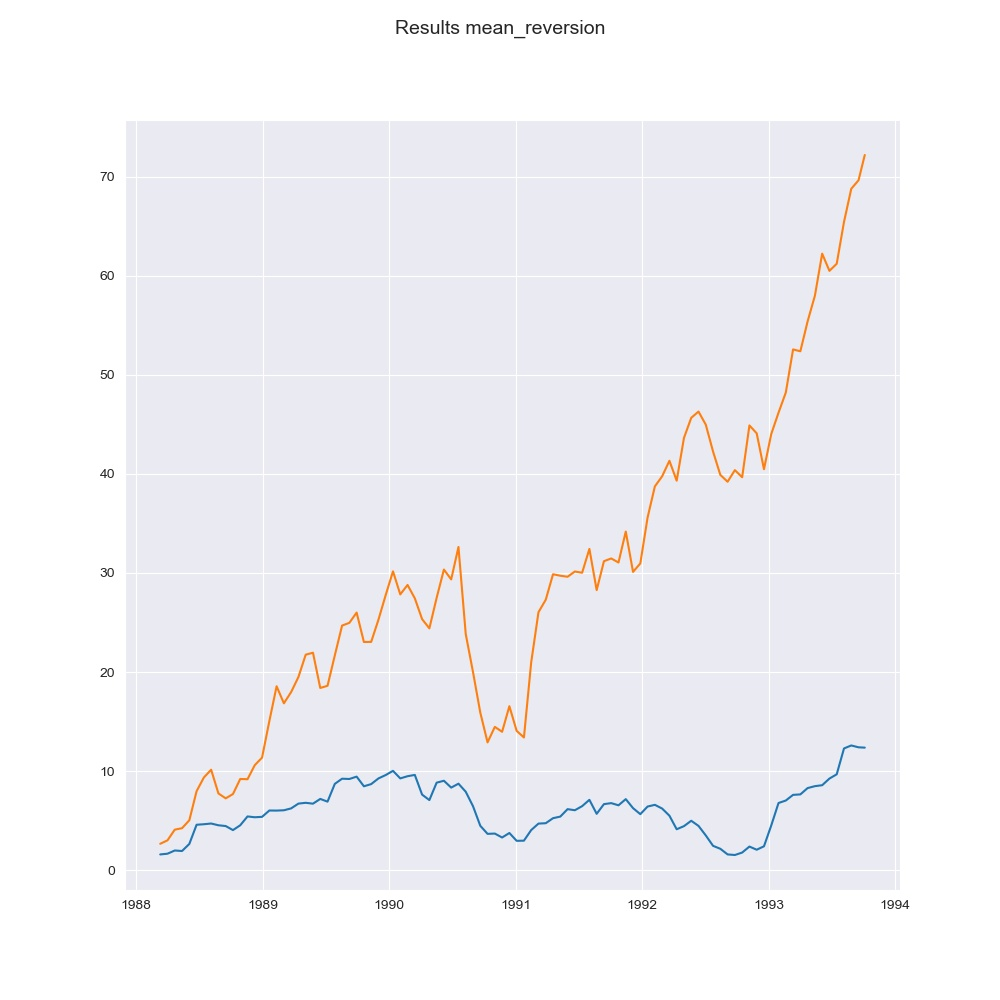
\includegraphics[width=0.48\textwidth]{../results/train_outliers_removed_mean_reversion_results.jpg}

    \caption{Results first 1500 obs, Assets 2 and 25 removed, baseline in orange}
    \label{3}
  
\end{figure}{}


\section{Results for the whole period}
Results for the whole data set are shown in Figure \ref{4}. Again, momentum trading and mean reversion perform worse than buy-and-hold. 

\begin{figure}[h!]
    %\figuretitle{Stock Prices}
    \centering
    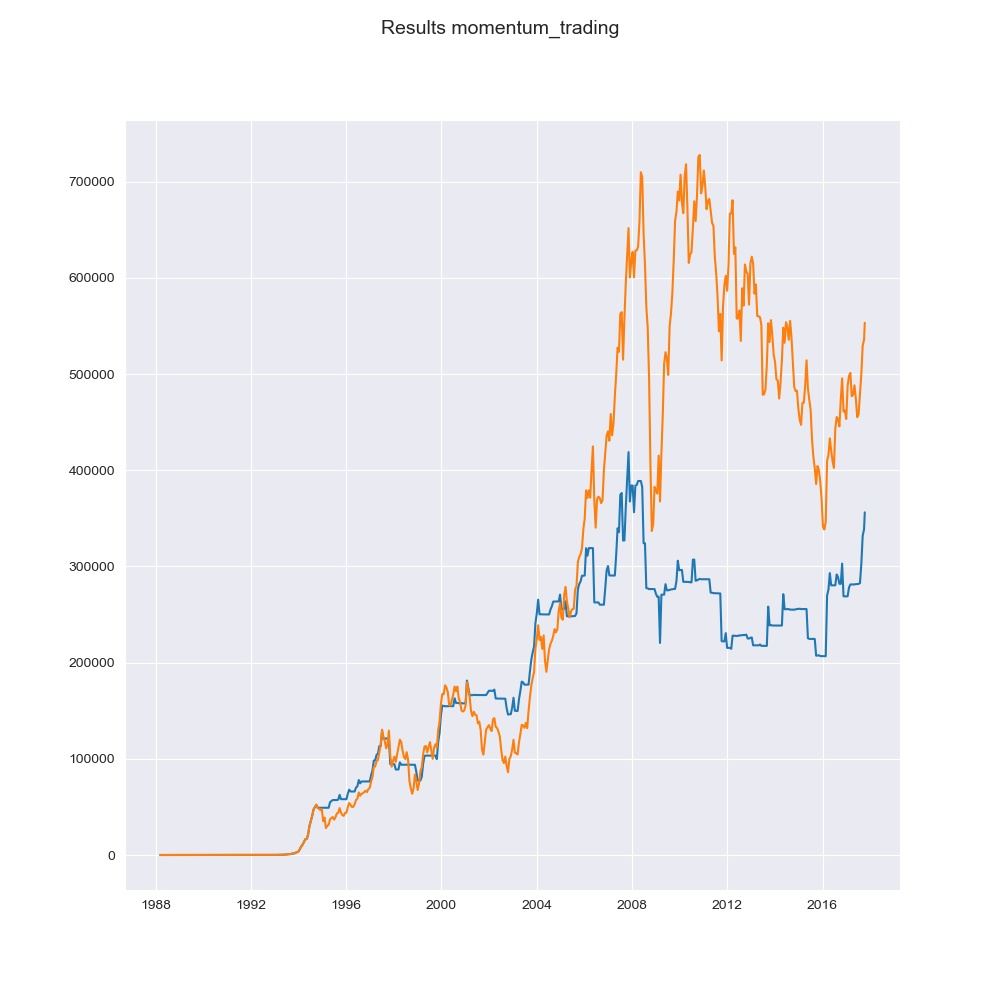
\includegraphics[width=0.48\textwidth]{../results/results_full_ts/momentum_trading_results.jpg}
    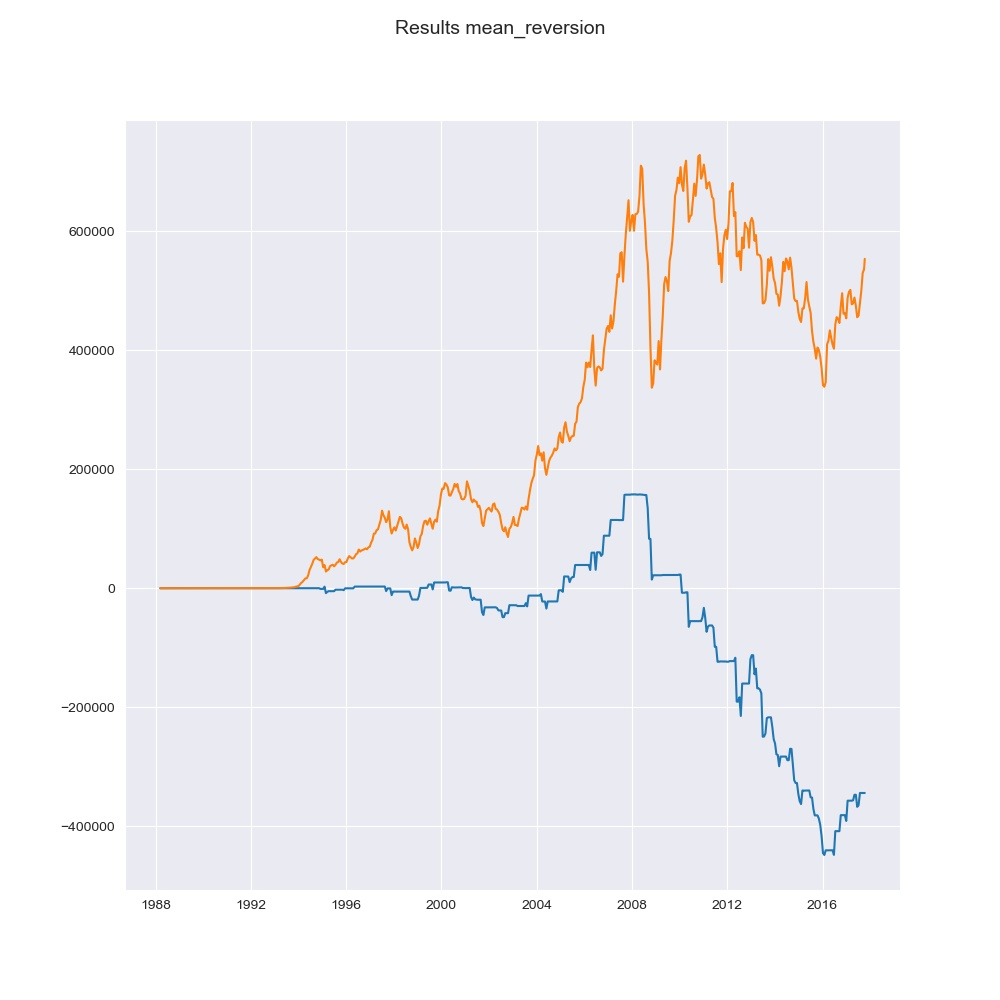
\includegraphics[width=0.48\textwidth]{../results/results_full_ts/mean_reversion_results.jpg}

    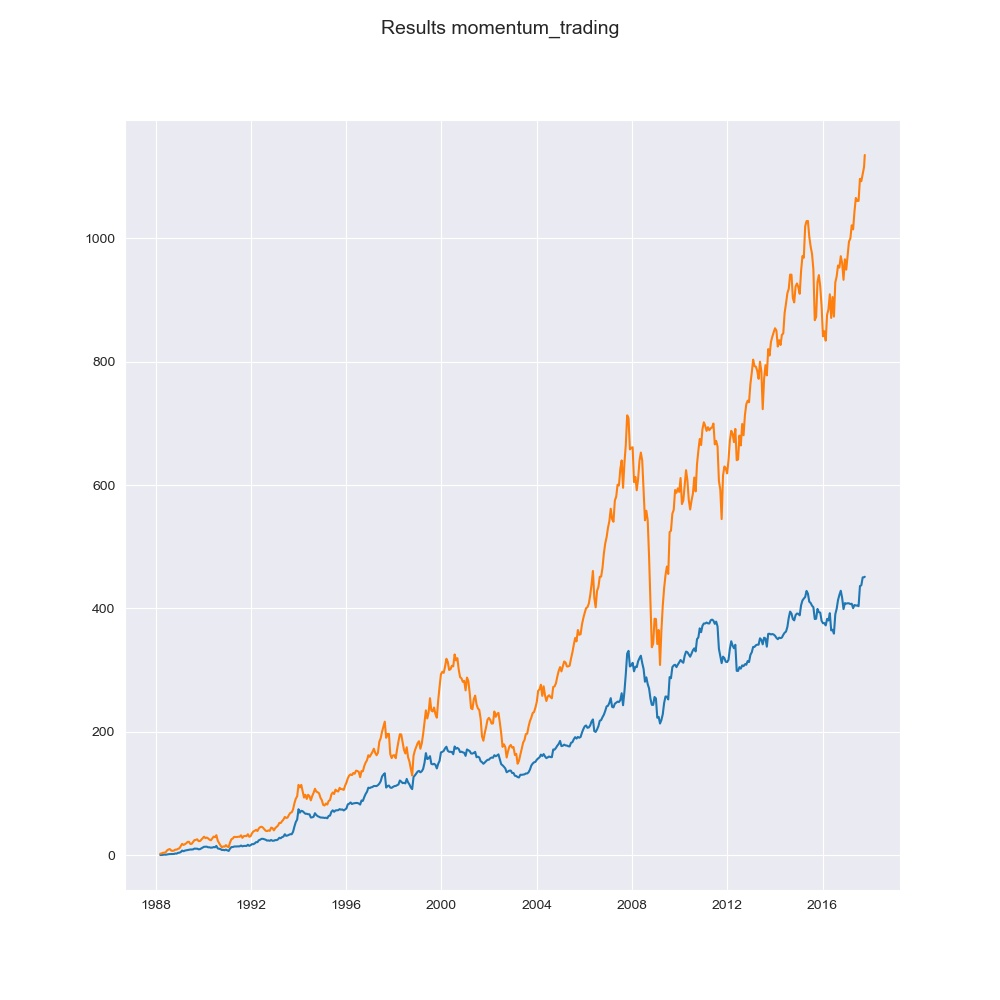
\includegraphics[width=0.48\textwidth]{../results/results_full_ts/outlier_removed_momentum_trading_results.jpg}
    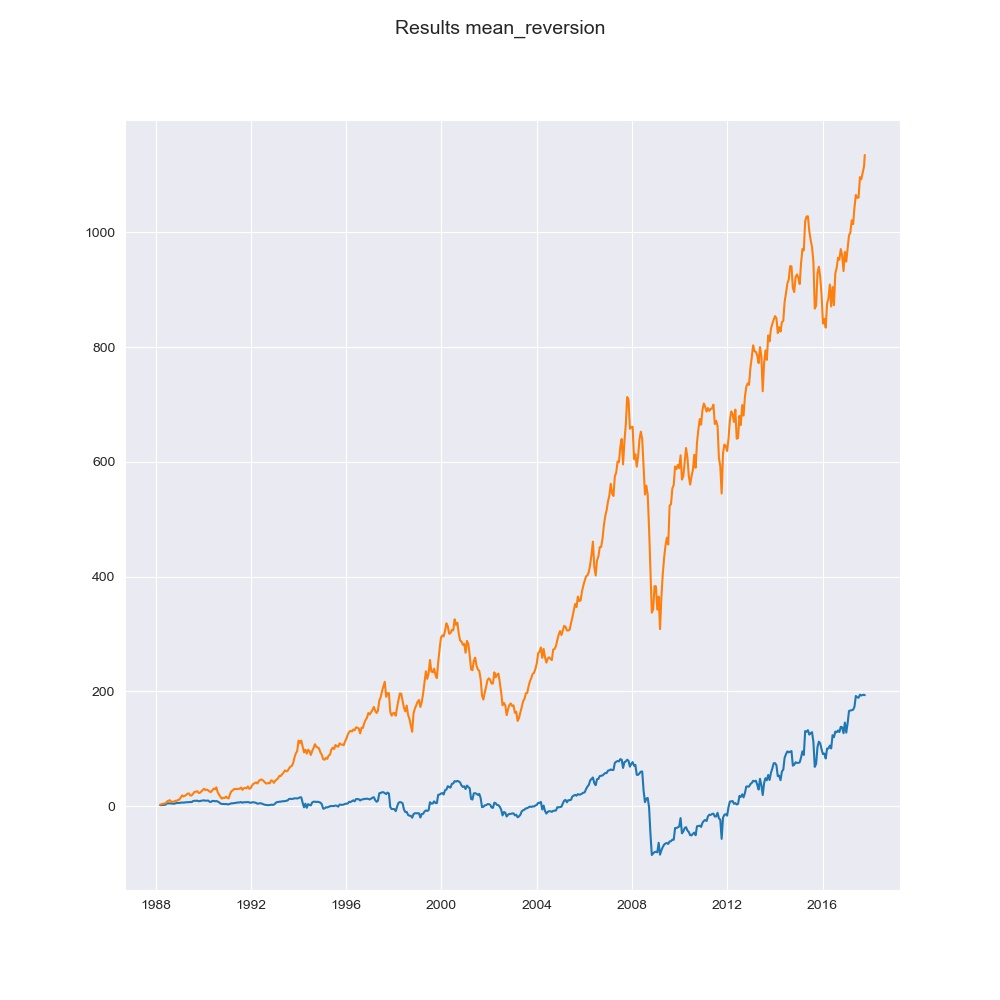
\includegraphics[width=0.48\textwidth]{../results/results_full_ts/outlier_removed_mean_reversion_results.jpg}

    \caption{Results full data set, baseline in orange. Second row: Assets 2 and 25 removed}
    \label{4}
  
\end{figure}{}


\chapter{Code}
The code and all the plots are available on https://github.com/nikosbosse/applicationexercise.

\chapter{Further Considerations}
The trading strategies proposed are in many ways not optimal and not optimized. To a certain extent this is intentional in order to avoid overfitting. But nevertheless there are many parameters to be tuned and ways in which the model could be extended. The trading frequency is one such parameter that could be chosen much shorter or much longer. Especially the time-series based forecasts could work better over a shorter, e.g. daily horizon. This can easily be changed, it just needs more computational power and time. 

\section{Extensions}
Other means of predictions could be used, i.e. vector time series models or machine learning approaches like XGBoost or LightGBM. 
